\chaptercustom{5}{KẾT QUẢ VÀ ĐÁNH GIÁ}
\setcounter{section}{5}
\setcounter{equation}{0}
Chương này trình bày kết quả cho từng câu hỏi Q1--Q3. Với mỗi câu hỏi, giá trị dự đoán từ mô hình giải tích ở Chương~4 được đặt cạnh cột số đo trên Mininet.

\textbf{Nguồn gốc số liệu.} Giá trị ``Mô hình'' tính bằng \texttt{code/model.py}. Giá trị ``Đo'' lấy từ Mininet 2.3.0 chạy trên Ubuntu 22.04 (WSL2), bằng \texttt{run\_experiments.py} và \texttt{summarize.py}: mỗi điểm là trung bình của 9 vòng (bỏ vòng 1), độ lệch chuẩn tính trên chính 9 vòng đó.

Cần lưu ý cách server ghi thời gian (\texttt{fl\_server.py}): $T_{down}$ tính tới khi Edge Node \emph{cuối cùng} nhận xong mô hình, còn $T_{up}$ tính từ lúc Edge Node \emph{đầu tiên} train xong. Nếu các luồng tải xuống không kết thúc cùng lúc, nút xong sớm bắt đầu upload trong khi nút khác còn đang tải xuống; hai pha chồng lên nhau, nên số đo $T_{round}$ có thể nhỏ hơn $T_{down} + T_{train} + T_{up}$, và $T_{up}$ đo được bao gồm cả độ lệch thời điểm kết thúc tải xuống giữa các nút.

\subsection{Kiểm tra môi trường}
Trước khi đo, nhóm dựng topo bằng \texttt{tools/sanity.py} (giống \texttt{topo.py}, thêm bước tắt TSO/GSO/GRO như \texttt{run\_experiments.py}) rồi chạy ping và iperf trong Mininet CLI. Hình~\ref{fig:sanity100} và Hình~\ref{fig:sanity20} là ảnh chụp terminal của hai lần chạy, với WAN 100 Mbps và 20 Mbps.

\begin{figure}[H]
    \centering
    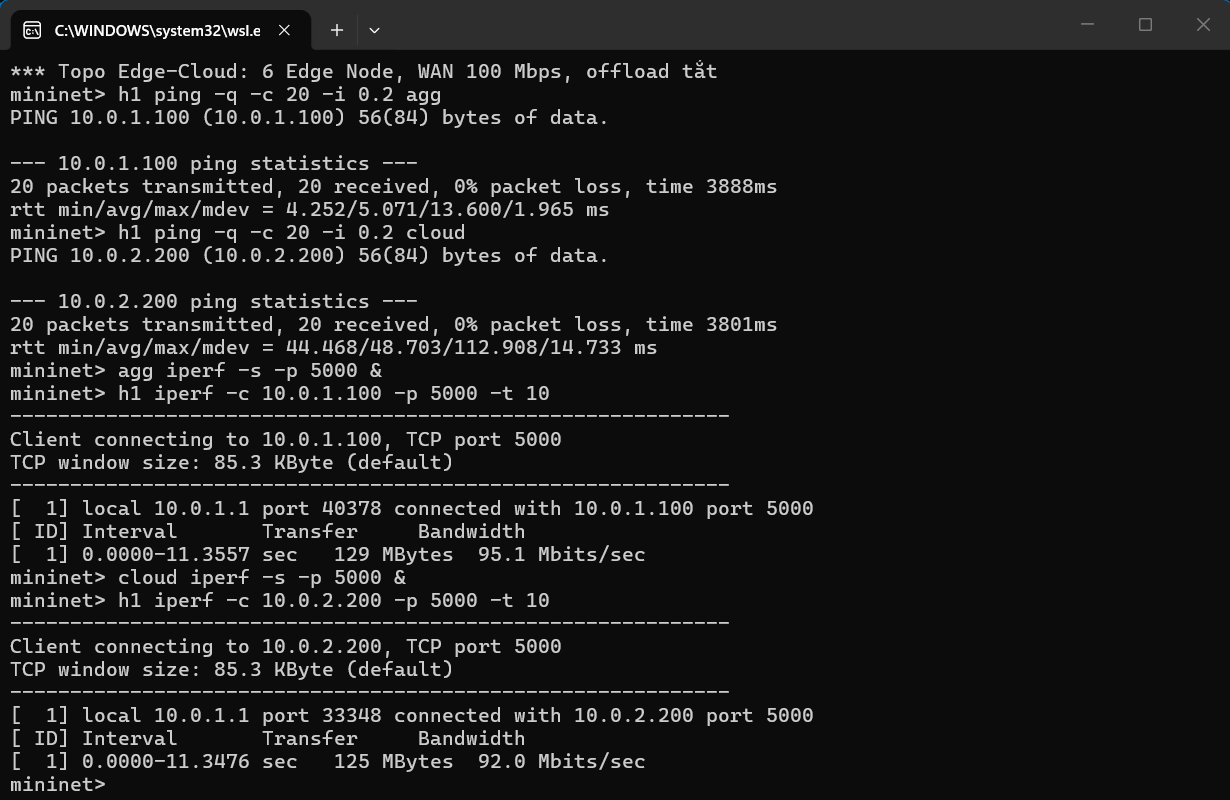
\includegraphics[width=0.85\textwidth]{Images/run/sanity_wan100.png}
    \caption{Kiểm tra RTT và thông lượng trong Mininet CLI, WAN 100 Mbps}
    \label{fig:sanity100}
\end{figure}

\begin{figure}[H]
    \centering
    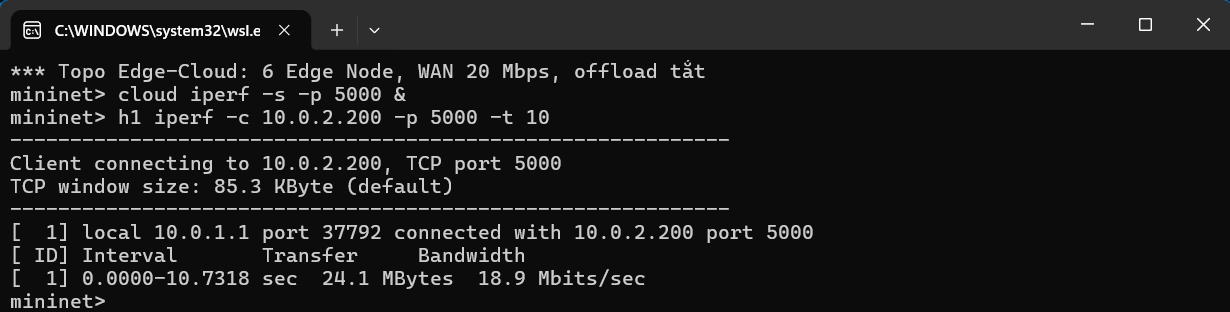
\includegraphics[width=0.85\textwidth]{Images/run/sanity_wan20.png}
    \caption{Kiểm tra thông lượng tới Cloud Server, WAN 20 Mbps}
    \label{fig:sanity20}
\end{figure}

RTT đo bằng 20 gói \texttt{ping} cách nhau 0{,}2~s; \texttt{iperf} chạy 10~s trên cổng 5000, cổng duy nhất firewall của \texttt{r1} cho phép tới Cloud Server. RTT nhỏ nhất là 4{,}25~ms tới \texttt{agg} và 44{,}47~ms tới \texttt{cloud}, khớp với giá trị kỳ vọng 4 và 44~ms. RTT trung bình (5{,}07 và 48{,}70~ms) cao hơn vì gói đầu tiên phải chờ phân giải ARP (13{,}6 và 112{,}9~ms). Thông lượng iperf là 95{,}1 Mbps tới \texttt{agg}, 92{,}0 Mbps tới \texttt{cloud} qua WAN 100 Mbps và 18{,}9 Mbps qua WAN 20 Mbps, đều không thấp hơn quá 4\% so với giới hạn $\eta B$ (95{,}6 và 19{,}1 Mbps). Cấu hình băng thông và độ trễ của topo vì vậy có hiệu lực.

Hình~\ref{fig:runk1} là ảnh chụp một lần chạy thử kịch bản K1 với $N = 4$ và 5 vòng, gõ trực tiếp trong Mininet CLI: bốn Edge Node chạy nền, Aggregator in thời gian từng vòng rồi ghi log CSV. $T_{round}$ của vòng 2--5 là 7{,}27--7{,}46~s, khớp với giá trị trung bình 7{,}333~s ở Bảng~\ref{tab:q1}.

\begin{figure}[H]
    \centering
    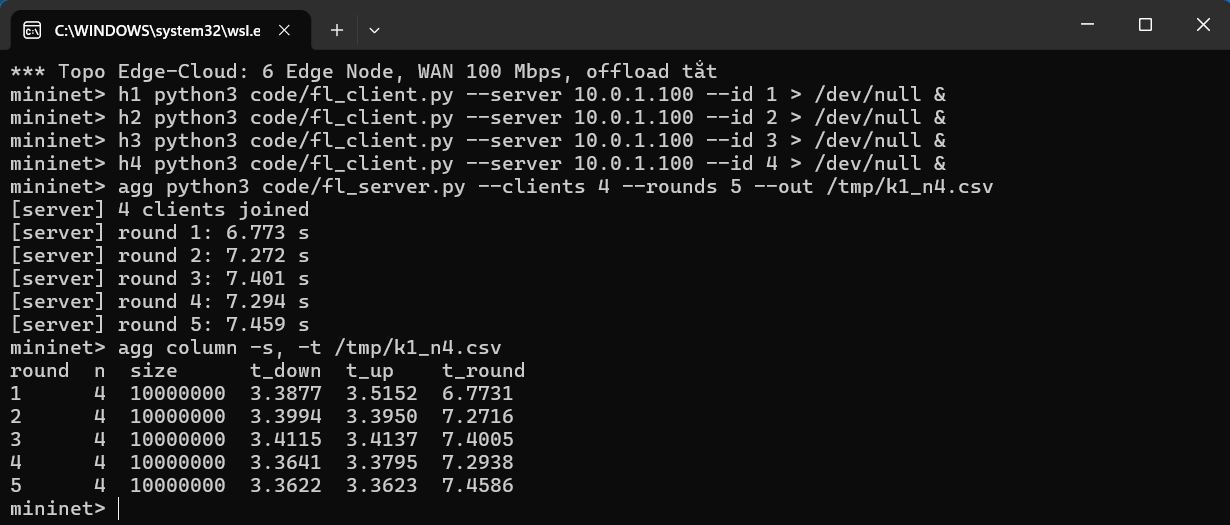
\includegraphics[width=0.85\textwidth]{Images/run/run_k1_n4.png}
    \caption{Một lần chạy kịch bản K1, $N = 4$, 5 vòng: log của Aggregator và file CSV}
    \label{fig:runk1}
\end{figure}

\subsection{Q1 -- Ảnh hưởng của số Edge Node}
Bảng~\ref{tab:q1} và Hình~\ref{fig:q1} cho thời gian các pha của kịch bản K1 (Aggregator tại biên, 10 MB mỗi chiều).

\begin{table}[H]
    \centering
    \caption{Thời gian các pha theo số Edge Node, kịch bản K1 (giây)}
    \label{tab:q1}
    \begin{tabular}{c c c c c c}
        \toprule
        \multirow{2}{*}{$N$} & \multicolumn{3}{c}{\textbf{Mô hình}} & \multicolumn{2}{c}{\textbf{Đo}} \\
        \cmidrule(lr){2-4} \cmidrule(lr){5-6}
        & $T_{down}$ & $T_{up}$ & $T_{round}$ & $T_{round}$ & độ lệch chuẩn \\
        \midrule
        2 & 1,677 & 1,677 & 4,353 & 4,446 & 0,036 \\
        3 & 2,512 & 2,512 & 6,024 & 5,882 & 0,114 \\
        4 & 3,348 & 3,348 & 7,696 & 7,333 & 0,117 \\
        5 & 4,184 & 4,184 & 9,369 & 8,566 & 0,207 \\
        6 & 5,021 & 5,021 & 11,042 & 9,943 & 0,311 \\
        \bottomrule
    \end{tabular}
\end{table}

\begin{figure}[H]
    \centering
    \begin{tikzpicture}
        \begin{axis}[
            width=0.85\textwidth, height=7cm,
            xlabel={Số Edge Node $N$}, ylabel={Thời gian (s)},
            xmin=1.8, xmax=6.2, xtick={2,3,4,5,6},
            ymin=0, grid=major, grid style={gray!25},
            legend pos=north west, legend cell align=left,
            restrict x to domain=2:6,
        ]
            \addplot[thick, blue, mark=*] table[x=n, y=t_round, col sep=comma] {data/model_edge_10MB.csv};
            \addlegendentry{$T_{round}$ (mô hình)}
            \addplot[thick, blue!50, mark=square, dashed] table[x=n, y=t_up, col sep=comma] {data/model_edge_10MB.csv};
            \addlegendentry{$T_{up}$ (mô hình)}
            \addplot[red, mark=triangle*, error bars/.cd, y dir=both, y explicit]
                table[x=n, y=t_round, y error=t_round_sd, col sep=comma] {data/measured_K1_edge_full.csv};
            \addlegendentry{$T_{round}$ (đo)}
        \end{axis}
    \end{tikzpicture}
    \caption{Thời gian một vòng theo số Edge Node, Aggregator tại biên, 10 MB}
    \label{fig:q1}
\end{figure}

\textbf{Nhận xét.} Theo mô hình, mỗi Edge Node thêm vào làm mỗi pha dài thêm khoảng 0{,}84~s, tức $T_{round}$ tăng khoảng 1{,}67~s. Từ $N = 2$ lên $N = 6$, $T_{round}$ tăng từ 4{,}35~s lên 11{,}04~s (gấp 2{,}5 lần), trong khi phần huấn luyện cố định 1~s không đổi. Nguyên nhân là link 100 Mbps tới Aggregator đã bão hoà ngay từ $N = 1$: thêm Edge Node không làm tổng thông lượng tăng mà chỉ chia nhỏ phần của mỗi nút ($B/N$, còn khoảng 16 Mbps mỗi nút khi $N = 6$). Trong khi đó, mỗi link truy nhập của Edge Node có 100 Mbps nhưng chỉ dùng được $1/N$.

Bảng~\ref{tab:q1thr} cho thông lượng của pha upload, tính bằng $8NS/T_{up}$. Thông lượng gộp đứng yên ở khoảng 95{,}6 Mbps (giới hạn $\eta B$ của link 100 Mbps), còn phần của mỗi nút giảm theo $1/N$.

\begin{table}[H]
    \centering
    \caption{Thông lượng ứng dụng của pha upload, kịch bản K1 (Mbps)}
    \label{tab:q1thr}
    \begin{tabular}{c c c c c}
        \toprule
        \multirow{2}{*}{$N$} & \multicolumn{2}{c}{\textbf{Mô hình}} & \multicolumn{2}{c}{\textbf{Đo}} \\
        \cmidrule(lr){2-3} \cmidrule(lr){4-5}
        & gộp & mỗi nút & gộp & mỗi nút \\
        \midrule
        2 & 95,4 & 47,7 & 91,2 & 45,6 \\
        3 & 95,6 & 31,9 & 93,1 & 31,0 \\
        4 & 95,6 & 23,9 & 94,8 & 23,7 \\
        5 & 95,6 & 19,1 & 94,4 & 18,9 \\
        6 & 95,6 & 15,9 & 92,1 & 15,4 \\
        \bottomrule
    \end{tabular}
\end{table}

Cột ``Đo'' lấy từ cột \texttt{thr\_mbps} do \texttt{summarize.py} tính, và có thể đối chiếu với \emph{Statistics $\rightarrow$ Conversations} trên Wireshark. Link nghẽn vì vậy là link \texttt{s1}--\texttt{agg}, tức \emph{giao diện mạng của nút tổng hợp}; link truy nhập của mỗi Edge Node còn dư $(N-1)/N$ băng thông. Muốn rút ngắn vòng khi tăng số nút, phải tăng băng thông vào Aggregator, giảm kích thước dữ liệu (Q2), hoặc chia tải cho nhiều Aggregator (tổng hợp phân cấp).

\textbf{Đối chiếu với số đo.} (1) Thông lượng gộp đo được 91--95 Mbps ở mọi $N$, khớp với nhận định link \texttt{s1}--\texttt{agg} bão hoà. (2) $T_{down}$ đo tăng từ 1{,}717~s ($N = 2$) lên 5{,}159~s ($N = 6$), tức khoảng 0{,}86~s mỗi nút, gần với hệ số góc 0{,}84~s của mô hình. (3) Tuy vậy $T_{round}$ đo chỉ tăng khoảng 1{,}37~s mỗi nút (thay vì 1{,}67~s) và từ $N = 3$ trở đi nhỏ hơn mô hình, tới 1{,}1~s ở $N = 6$ (9{,}94~s so với 11{,}04~s). Nguyên nhân là các pha chồng lên nhau: nút nhận xong mô hình sớm bắt đầu upload trong khi nút khác còn tải xuống, nên $T_{round}$ nhỏ hơn $T_{down} + 1 + T_{up} = 11{,}37$~s; mô hình giả thiết các pha nối tiếp nhau. (4) Độ lệch chuẩn tăng từ 0{,}036~s lên 0{,}311~s khi $N$ tăng, cho thấy các luồng chia băng thông kém đều hơn khi có nhiều nút.

\subsection{Q2 -- Gửi toàn bộ mô hình so với gradient nén}
Câu hỏi Q2 được xét trên ba chỉ số: thời gian pha upload, thời gian cả vòng và RTT khi có tải.

\subsubsection{Thời gian truyền chiều lên}
Bảng~\ref{tab:q2} so sánh $T_{up}$ khi gửi 10 MB và 1 MB, ở cả hai vị trí Aggregator.

\begin{table}[H]
    \centering
    \caption{Thời gian pha upload $T_{up}$ (giây) và hệ số giảm khi nén 1/10, giá trị mô hình}
    \label{tab:q2}
    \begin{tabular}{c c c c c c c}
        \toprule
        \multirow{2}{*}{$N$} & \multicolumn{3}{c}{\textbf{Edge (RTT 4 ms)}} & \multicolumn{3}{c}{\textbf{Cloud (RTT 44 ms, 100 Mbps)}} \\
        \cmidrule(lr){2-4} \cmidrule(lr){5-7}
        & 10 MB & 1 MB & giảm & 10 MB & 1 MB & giảm \\
        \midrule
        1 & 0,843 & 0,090 & 9,4$\times$ & 1,046 & 0,293 & 3,6$\times$ \\
        2 & 1,677 & 0,171 & 9,8$\times$ & 1,840 & 0,334 & 5,5$\times$ \\
        3 & 2,512 & 0,253 & 9,9$\times$ & 2,653 & 0,394 & 6,7$\times$ \\
        4 & 3,348 & 0,337 & 9,9$\times$ & 3,471 & 0,460 & 7,5$\times$ \\
        5 & 4,184 & 0,420 & 10,0$\times$ & 4,294 & 0,530 & 8,1$\times$ \\
        6 & 5,021 & 0,504 & 10,0$\times$ & 5,122 & 0,605 & 8,5$\times$ \\
        \bottomrule
    \end{tabular}
\end{table}

\begin{figure}[H]
    \centering
    \begin{tikzpicture}
        \begin{axis}[
            width=0.85\textwidth, height=7cm,
            xlabel={Số Edge Node $N$}, ylabel={$T_{up}$ (s)},
            xmin=0.8, xmax=6.2, xtick={1,...,6},
            ymode=log, log basis y=10,
            grid=major, grid style={gray!25},
            legend style={at={(0.5,-0.3)}, anchor=north, legend columns=2}, legend cell align=left,
        ]
            \addplot[thick, blue, mark=*] table[x=n, y=t_up, col sep=comma] {data/model_edge_10MB.csv};
            \addlegendentry{Edge, 10 MB}
            \addplot[thick, blue, mark=o, dashed] table[x=n, y=t_up, col sep=comma] {data/model_edge_1MB.csv};
            \addlegendentry{Edge, 1 MB}
            \addplot[thick, orange, mark=square*] table[x=n, y=t_up, col sep=comma] {data/model_cloud_10MB.csv};
            \addlegendentry{Cloud, 10 MB}
            \addplot[thick, orange, mark=square, dashed] table[x=n, y=t_up, col sep=comma] {data/model_cloud_1MB.csv};
            \addlegendentry{Cloud, 1 MB}
            \addplot[red, mark=triangle*] table[x=n, y=t_up, col sep=comma] {data/measured_K2_edge_comp.csv};
            \addlegendentry{Edge, 1 MB (đo)}
            \addplot[red!60!black, mark=diamond*] table[x=n, y=t_up, col sep=comma] {data/measured_K2_cloud_comp.csv};
            \addlegendentry{Cloud, 1 MB (đo)}
        \end{axis}
    \end{tikzpicture}
    \caption{Thời gian upload khi gửi toàn bộ mô hình và gradient nén (trục tung logarit)}
    \label{fig:q2}
\end{figure}

\textbf{Nhận xét.} Ở biên, nén 1/10 giảm $T_{up}$ gần đúng 10 lần, vì RTT chỉ 4~ms và slow start kết thúc sau 2 RTT; gần như toàn bộ thời gian là $d_{trans}$, tỷ lệ thuận với kích thước.

Qua WAN, mức giảm thấp hơn nhiều khi ít nút: chỉ 3{,}6 lần với $N = 1$. Một luồng gửi 1 MB phải qua khoảng 6 RTT slow start (264~ms) trước khi cửa sổ đủ lớn, trong khi $d_{trans}$ của 1 MB ở 100 Mbps chỉ khoảng 84~ms. Nén làm giảm $d_{trans}$ nhưng không giảm được số RTT. Khi $N$ tăng, tổng cửa sổ của $N$ luồng lấp đầy BDP nhanh hơn ($k^{*}$ nhỏ đi) và $d_{trans}$ lại chiếm ưu thế, nên mức giảm tiến dần về 10 lần.

Với thiết kế hệ thống, điều này có nghĩa là nén gradient có lợi nhất khi link chậm hoặc nhiều nút cùng chia link. Với ít nút qua WAN có RTT lớn, cần kết hợp thêm biện pháp ở tầng giao vận, ví dụ tắt \nolinkurl{tcp_slow_start_after_idle} để giữ $cwnd$ giữa các vòng, hoặc tăng IW.

Bảng~\ref{tab:q2meas} cho $T_{up}$ đo được của bốn kịch bản (K1, K2\_edge, K3\_cloud, K2\_cloud).

\begin{table}[H]
    \centering
    \caption{Thời gian pha upload $T_{up}$ (giây) và hệ số giảm khi nén 1/10, số đo}
    \label{tab:q2meas}
    \begin{tabular}{c c c c c c c}
        \toprule
        \multirow{2}{*}{$N$} & \multicolumn{3}{c}{\textbf{Edge}} & \multicolumn{3}{c}{\textbf{Cloud (100 Mbps)}} \\
        \cmidrule(lr){2-4} \cmidrule(lr){5-7}
        & 10 MB & 1 MB & giảm & 10 MB & 1 MB & giảm \\
        \midrule
        2 & 1,755 & 0,259 & 6,8$\times$ & 2,733 & 0,798 & 3,4$\times$ \\
        3 & 2,578 & 0,333 & 7,7$\times$ & 3,321 & 1,762 & 1,9$\times$ \\
        4 & 3,374 & 0,481 & 7,0$\times$ & 4,975 & 1,518 & 3,3$\times$ \\
        5 & 4,235 & 0,901 & 4,7$\times$ & 6,911 & 2,419 & 2,9$\times$ \\
        6 & 5,214 & 1,424 & 3,7$\times$ & 7,112 & 3,117 & 2,3$\times$ \\
        \bottomrule
    \end{tabular}
\end{table}

Số đo cho mức giảm thấp hơn mô hình, và khác mô hình ở chỗ mức giảm \emph{giảm dần} khi $N$ tăng (Edge: từ 6{,}8 xuống 3{,}7 lần). Lý do nằm ở cách đo đã nêu đầu chương: $T_{up}$ tính từ lúc nút đầu tiên train xong, nên bao gồm khoảng lệch giữa nút nhận xong mô hình 10 MB sớm nhất và muộn nhất. Khoảng lệch này không phụ thuộc kích thước bản cập nhật và tăng theo $N$; khi bản cập nhật chỉ còn 1 MB, nó chiếm phần lớn $T_{up}$. Qua WAN, sự chênh lệch giữa các luồng còn lớn hơn (độ lệch chuẩn tới 0{,}65~s ở K2\_cloud), nên mức giảm chỉ còn 1{,}9--3{,}4 lần. Nói cách khác, khi chiều lên đã được nén, sự không đều của pha tải xuống trở thành yếu tố quyết định thời gian chờ của Aggregator.

\subsubsection{Thời gian vòng khi chỉ nén chiều lên}
Vì mô hình toàn cục phát xuống vẫn là 10 MB, lợi ích trên toàn vòng nhỏ hơn lợi ích trên pha upload. Với $N = 6$ tại biên, $T_{round}$ giảm từ 11{,}04~s xuống $5{,}02 + 1 + 0{,}50 = 6{,}53$~s (giảm 41\%); tại Cloud 100 Mbps, từ 11{,}24~s xuống 6{,}73~s. Pha phát xuống trở thành phần chiếm ưu thế, gợi ý rằng bước tiếp theo nên là nén cả chiều xuống hoặc dùng multicast.

Số đo với $N = 6$: tại biên $T_{round}$ giảm từ 9{,}94~s (K1) xuống 6{,}17~s (K2\_edge), tức giảm 38\%; tại Cloud 100 Mbps giảm từ 11{,}80~s (K3\_cloud) xuống 7{,}52~s (K2\_cloud), tức giảm 36\%. Mức giảm trên toàn vòng gần với dự đoán của mô hình (41\% và 40\%), dù mức giảm của riêng pha upload thấp hơn nhiều.

\subsubsection{RTT khi có tải}
Trong lúc $N$ luồng cùng đẩy dữ liệu, hàng đợi tại cổng \texttt{s1} hướng tới Aggregator đầy dần. Với hàng đợi 200 gói, công thức~\eqref{eq:dqueue} ở Chương~2 cho độ trễ hàng đợi tối đa khoảng 24~ms, nên RTT đo bằng ping từ \texttt{h1} có thể tăng từ 4~ms lên gần 28~ms trong pha upload. Khi nén 1/10, thời gian hàng đợi bị đầy rút ngắn khoảng 10 lần, và với ít nút các luồng 1 MB có thể kết thúc trước khi hàng đợi kịp đầy. Bảng~\ref{tab:q2rtt} cho số đo.

\begin{table}[H]
    \centering
    \caption{RTT từ h1 tới Aggregator trong suốt lần đo, $N = 6$ (ms)}
    \label{tab:q2rtt}
    \begin{tabular}{l c c c}
        \toprule
        \textbf{Kịch bản} & \textbf{RTT rảnh} & \textbf{RTT trung bình khi có tải} & \textbf{RTT lớn nhất} \\
        \midrule
        Edge, 10 MB (K1) & 4,3 & 32,2 & 58,5 \\
        Edge, 1 MB (K2) & 4,3 & 35,9 & 54,1 \\
        Cloud, 10 MB (K3) & 44,5 & 62,0 & 95,3 \\
        Cloud, 1 MB (K2) & 44,5 & 63,3 & 92,9 \\
        \bottomrule
    \end{tabular}
\end{table}

RTT rảnh là RTT nhỏ nhất ở Hình~\ref{fig:sanity100}, không tính gói đầu chờ ARP. RTT khi có tải tính trên toàn bộ log \texttt{ping -i 0.2} của lần đo, gồm cả pha tải xuống và pha upload, vì log không ghi mốc thời gian để tách riêng từng pha.

RTT lớn nhất đo được (54--58~ms tại biên) vượt mức khoảng 28~ms dự đoán cho riêng hàng đợi chiều lên. Do các pha chồng lên nhau, có lúc hàng đợi 200 gói ở cả hai chiều của link \texttt{s1}--\texttt{agg} cùng đầy; $4 + 24 + 24 \approx 52$~ms, gần với giá trị đo. Nén chiều lên không làm giảm RTT trung bình (35{,}9~ms so với 32{,}2~ms tại biên), vì pha tải xuống 10 MB vẫn làm đầy hàng đợi chiều xuống trong phần lớn thời gian của vòng.

\subsection{Q3 -- Tổng hợp tại Edge so với tại Cloud}
\begin{figure}[H]
    \centering
    \begin{tikzpicture}
        \begin{axis}[
            width=0.85\textwidth, height=7cm,
            xlabel={Số Edge Node $N$}, ylabel={$T_{round}$ (s)},
            xmin=1.8, xmax=6.2, xtick={2,3,4,5,6},
            ymin=0, grid=major, grid style={gray!25},
            legend pos=north west, legend cell align=left,
            restrict x to domain=2:6,
        ]
            \addplot[thick, blue, mark=*] table[x=n, y=t_round, col sep=comma] {data/model_edge_10MB.csv};
            \addlegendentry{Edge (RTT 4 ms, 100 Mbps)}
            \addplot[thick, orange, mark=square*] table[x=n, y=t_round, col sep=comma] {data/model_cloud_10MB.csv};
            \addlegendentry{Cloud (RTT 44 ms, 100 Mbps)}
            \addplot[thick, red!70!black, mark=triangle*] table[x=n, y=t_round, col sep=comma] {data/model_cloud20_10MB.csv};
            \addlegendentry{Cloud (RTT 44 ms, 20 Mbps)}
            \addplot[blue, only marks, mark=x, mark size=4pt, forget plot] table[x=n, y=t_round, col sep=comma] {data/measured_K1_edge_full.csv};
            \addplot[orange, only marks, mark=x, mark size=4pt, forget plot] table[x=n, y=t_round, col sep=comma] {data/measured_K3_cloud_full.csv};
            \addplot[red!70!black, only marks, mark=x, mark size=4pt] table[x=n, y=t_round, col sep=comma] {data/measured_K3_cloud20_full.csv};
            \addlegendentry{Số đo (dấu $\times$, cùng màu)}
        \end{axis}
    \end{tikzpicture}
    \caption{Thời gian một vòng theo vị trí Aggregator, 10 MB mỗi chiều}
    \label{fig:q3}
\end{figure}

\begin{table}[H]
    \centering
    \caption{$T_{round}$ theo vị trí Aggregator (giây), giá trị mô hình và số đo}
    \label{tab:q3}
    \resizebox{\textwidth}{!}{%
    \begin{tabular}{c c c c c c c c c}
        \toprule
        \multirow{2}{*}{$N$} & \multicolumn{4}{c}{\textbf{Mô hình}} & \multicolumn{4}{c}{\textbf{Đo}} \\
        \cmidrule(lr){2-5} \cmidrule(lr){6-9}
        & Edge & Cloud 100M & chênh & Cloud 20M & Edge & Cloud 100M & chênh & Cloud 20M \\
        \midrule
        2 & 4,353 & 4,680 & 0,327 & 17,877 & 4,446 & 5,480 & 1,034 & 17,540 \\
        3 & 6,024 & 6,306 & 0,282 & 26,205 & 5,882 & 6,312 & 0,430 & 25,035 \\
        4 & 7,696 & 7,942 & 0,247 & 34,542 & 7,333 & 8,361 & 1,028 & 33,137 \\
        5 & 9,369 & 9,588 & 0,219 & 42,895 & 8,566 & 10,090 & 1,524 & 40,457 \\
        6 & 11,042 & 11,244 & 0,202 & 51,247 & 9,943 & 11,803 & 1,860 & 48,382 \\
        \bottomrule
    \end{tabular}}
\end{table}

\textbf{Nhận xét.} Khi băng thông WAN bằng băng thông nhánh biên, chênh lệch giữa Cloud và Edge chỉ còn 0{,}2--0{,}33~s mỗi vòng, tức 2--7\% $T_{round}$. Phần chênh này đến từ hai nguồn: slow start dài hơn (6 RTT $\times$ 44~ms thay vì 2 RTT $\times$ 4~ms, xảy ra ở cả hai pha) và thêm nửa RTT lan truyền cho mỗi pha. Bắt tay chỉ xảy ra một lần khi kết nối nên không góp vào các vòng sau. Chênh lệch giảm dần khi $N$ tăng vì tổng cửa sổ của nhiều luồng lấp đầy BDP sau ít RTT hơn.

Khi WAN chỉ có 20 Mbps, $T_{round}$ gấp khoảng 4{,}6 lần so với Edge ở $N = 6$ (51{,}2~s so với 11{,}0~s). Phần chênh do RTT (khoảng 0{,}2~s) lúc này nhỏ hơn 1\% so với phần chênh do băng thông.

\textbf{Đối chiếu với số đo.} Với WAN 20 Mbps, số đo bám sát mô hình (sai khác dưới 6\%), và Cloud chậm hơn Edge 4{,}9 lần ở $N = 6$ (48{,}4~s so với 9{,}9~s). Với WAN 100 Mbps, Cloud chậm hơn Edge 0{,}43--1{,}86~s mỗi vòng, lớn hơn nhiều so với 0{,}2--0{,}33~s của mô hình, và chênh lệch có xu hướng \emph{tăng} theo $N$ thay vì giảm. Khi tổng cửa sổ của $N$ luồng vượt BDP của đường 44~ms, hàng đợi 200 gói tại \texttt{r1} tràn, CUBIC giảm cửa sổ rồi tăng lại chậm theo RTT lớn; mô hình không tính hiện tượng này. RTT khi có tải lên tới 95~ms (Bảng~\ref{tab:q2rtt}) xác nhận hàng đợi chặng WAN thường xuyên đầy. Dù vậy, kết luận định tính không đổi: với WAN rộng, phần chênh giữa Edge và Cloud chỉ khoảng 7--23\% $T_{round}$.

Như vậy câu trả lời cho Q3 phụ thuộc vào băng thông chặng WAN: nếu WAN đủ rộng, lợi ích của tổng hợp tại biên đối với khối 10 MB là nhỏ và chủ yếu do slow start; nếu WAN hẹp hơn LAN biên, tổng hợp tại biên rút ngắn vòng nhiều lần. Đây cũng là lập luận của kiến trúc phân cấp \cite{liu2020hierfavg}: tổng hợp nhiều lần ở biên, chỉ gửi một bản lên cloud, thay vì $N$ bản.

\subsection{Phân tích gói tin}
Các file \texttt{.pcap} được bắt trong một lần chạy riêng của K1 và K3 (WAN 100 Mbps) với $N = 4$, 3 vòng (Hình~\ref{fig:ws-syn} đến Hình~\ref{fig:ws-router} ở Chương~3). $T_{round}$ của lần chạy này là 6{,}8--7{,}6~s với K1 và 7{,}8--11{,}9~s với K3, cùng khoảng với số đo ở Bảng~\ref{tab:q3}. Đối chiếu với lý thuyết:
\begin{itemize}
    \item \textbf{Kích thước đoạn.} Gói SYN mang MSS 1460 (Hình~\ref{fig:ws-syn}); gần như mọi đoạn có dữ liệu dài 1448 byte, tức $1460 - 12$ byte tuỳ chọn Timestamps, đúng như giả thiết khi tính $\eta$ ở Chương~3.
    \item \textbf{Header FLSync.} Đoạn đầu của mỗi thông điệp là một đoạn 20 byte bắt đầu bằng \texttt{46 4C 53 59} (Hình~\ref{fig:ws-hdr}).
    \item \textbf{Slow start lặp lại ở mỗi vòng.} Trong 0{,}7~s đầu vòng 2 của luồng \texttt{cloud} $\rightarrow$ \texttt{h1} (Hình~\ref{fig:ws-stevens}), dữ liệu đi theo từng loạt cách nhau 45--51~ms, tức một RTT. Số gói mỗi loạt là 10, 18, 38, 76, 110, rồi giữ ở 115--121 gói. Loạt đầu 10 gói khớp với IW = 10 \cite{rfc6928}, và kích thước loạt gần gấp đôi sau mỗi RTT. Như vậy dù kết nối TCP được giữ từ vòng 1, sau 1~s nghỉ huấn luyện $cwnd$ bị đặt lại và luồng phải qua 4 RTT slow start, đúng với dự đoán ở Chương~2 về \nolinkurl{tcp_slow_start_after_idle}. Số RTT slow start (4) ít hơn con số khoảng 6 RTT tính cho một luồng đơn, vì với $N = 4$ mỗi luồng chỉ cần lấp đầy 1/4 BDP; kích thước loạt ổn định khoảng 170~KB mỗi RTT tương ứng khoảng 29 Mbps, gần phần chia đều $95/4$ Mbps.
    \item \textbf{Chia băng thông giữa các luồng.} Theo \texttt{tshark -z io,stat,1}, tổng tải tin trên \texttt{agg-eth0} giữ ở khoảng 11{,}8 MB/s (khoảng 94--95 Mbps) trong mọi giây có truyền, trừ các giây rơi vào khoảng nghỉ huấn luyện. Nhưng phần của từng luồng dao động mạnh từ 0 đến 8{,}2 MB/s, trong khi phần chia đều chỉ khoảng 2{,}95 MB/s (Hình~\ref{fig:ws-io}). Ở khoảng thời gian 1~s, các luồng không chia đều $B/N$: có lúc một luồng chiếm gần hết link trong khi luồng khác gần như dừng. Đây là bằng chứng trực tiếp cho giải thích ở Q1 và Q2 rằng các luồng kết thúc lệch nhau, làm các pha chồng lên nhau và làm $T_{up}$ đo được chứa cả khoảng chờ nút chậm nhất.
    \item \textbf{Mất gói tại hàng đợi.} Wireshark đánh dấu 343 gói \emph{TCP Retransmission} trên \texttt{agg-eth0} (K1) và 338 gói trên \texttt{cloud-eth0} (K3), trên tổng khoảng 254\,000 gói mỗi file (khoảng 0{,}13\%). Trên I/O Graph, cột \emph{TCP Errors} cao nhất rơi vào giây thứ 11, cùng lúc một luồng tăng vọt lên khoảng 9 kgói/s. Như vậy hàng đợi 200 gói có tràn, và mất gói xảy ra theo đợt khi một luồng tăng tốc đột ngột. Riêng loạt slow start vòng 2 ở Hình~\ref{fig:ws-stevens} không có gói truyền lại nào.
\end{itemize}

\subsection{Kết luận chương}
Số đo trên Mininet xác nhận các xu hướng chính của mô hình giải tích, với một số sai khác có giải thích được. (Q1) Thời gian vòng tăng tuyến tính theo số Edge Node do link tới Aggregator bão hoà ở 91--95 Mbps; độ dốc đo được khoảng 1{,}37~s mỗi nút, thấp hơn 1{,}67~s của mô hình vì các pha tải xuống và upload chồng lên nhau. (Q2) Nén 1/10 chiều lên giảm $T_{round}$ khoảng 36--38\% ở $N = 6$, gần với mô hình; nhưng mức giảm của riêng pha upload chỉ 3{,}7--7{,}7 lần tại biên và 1{,}9--3{,}4 lần qua WAN, vì thời gian chờ do các luồng tải xuống kết thúc không đều chiếm phần lớn khi bản cập nhật đã nhỏ. (Q3) Với WAN 20 Mbps, Cloud chậm hơn Edge khoảng 4{,}9 lần, khớp với mô hình; với WAN 100 Mbps, Cloud chậm hơn 0{,}43--1{,}86~s mỗi vòng, lớn hơn mô hình do mất gói tại hàng đợi chặng WAN.

\cleardoublepage
